\section{Étude d'ablation}
\label{sec:ablation}

\subsection{Comparaison des configurations}

Le Tableau~\ref{tab:ablation} présente les résultats de test (top-1,
top-5, perte, nombre de paramètres) pour les 12 configurations
entraînées : ResNet-50 (jeu complet et sous-échantillons), ViT
pré-entraîné (patch16 et patch32), et ViT entraîné from scratch (jeu
complet et sous-échantillons, patch16 et patch32).

\begin{table}[t]
  \centering
  \caption{Résultats de test pour l'ensemble des configurations entraînées.}
  \label{tab:ablation}
  \small
  \begin{tabular}{lccc}
    \toprule
    Configuration & Top-1 & Top-5 & Params \\
    \midrule
    ResNet-50 (100\,\%)          & 71{,}9\,\% & 93{,}6\,\% & 23{,}9M \\
    ResNet-50 (50\,\%)           & 48{,}7\,\% & 81{,}1\,\% & 23{,}9M \\
    ResNet-50 (25\,\%)           & 23{,}5\,\% & 48{,}9\,\% & 23{,}9M \\
    ResNet-50 (10\,\%)           & 5{,}1\,\%  & 14{,}0\,\% & 23{,}9M \\
    \midrule
    ViT pré-entraîné (patch32)   & 53{,}9\,\% & 83{,}5\,\% & 22{,}6M \\
    ViT pré-entraîné (patch16)   & 9{,}9\,\%  & 25{,}4\,\% & 21{,}7M \\
    \midrule
    ViT scratch (100\,\%)        & 1{,}1\,\%  & 4{,}8\,\%  & 11{,}1M \\
    ViT scratch (50\,\%)         & 2{,}2\,\%  & 7{,}1\,\%  & 11{,}1M \\
    ViT scratch (25\,\%)         & 1{,}0\,\%  & 4{,}9\,\%  & 11{,}1M \\
    ViT scratch (10\,\%)         & 1{,}1\,\%  & 4{,}5\,\%  & 11{,}1M \\
    ViT scratch (patch16, sans aug.) & 2{,}1\,\% & 9{,}0\,\% & 11{,}1M \\
    ViT scratch (patch32)        & 2{,}0\,\%  & 8{,}5\,\%  & 11{,}9M \\
    \bottomrule
  \end{tabular}
\end{table}

\subsection{Sensibilité à la quantité de données}

La Figure~\ref{fig:data_hungry} illustre la sensibilité de ResNet-50 et
du ViT from scratch à la fraction du jeu d'entraînement utilisée.
ResNet-50 présente une croissance monotone et régulière de
l'accuracy avec la quantité de données (5{,}1\,\% à 10\,\%, jusqu'à
71{,}9\,\% à 100\,\%), cohérente avec son biais inductif convolutif qui
lui permet d'extraire une structure utile même à partir de peu
d'exemples. Le ViT from scratch, à l'inverse, reste bloqué à un niveau
proche du hasard (0{,}5\,\% attendu pour 200 classes) quelle que soit
la fraction de données utilisée, sans amélioration significative entre
10\,\% et 100\,\%.

\begin{figure}[t]
  \centering
  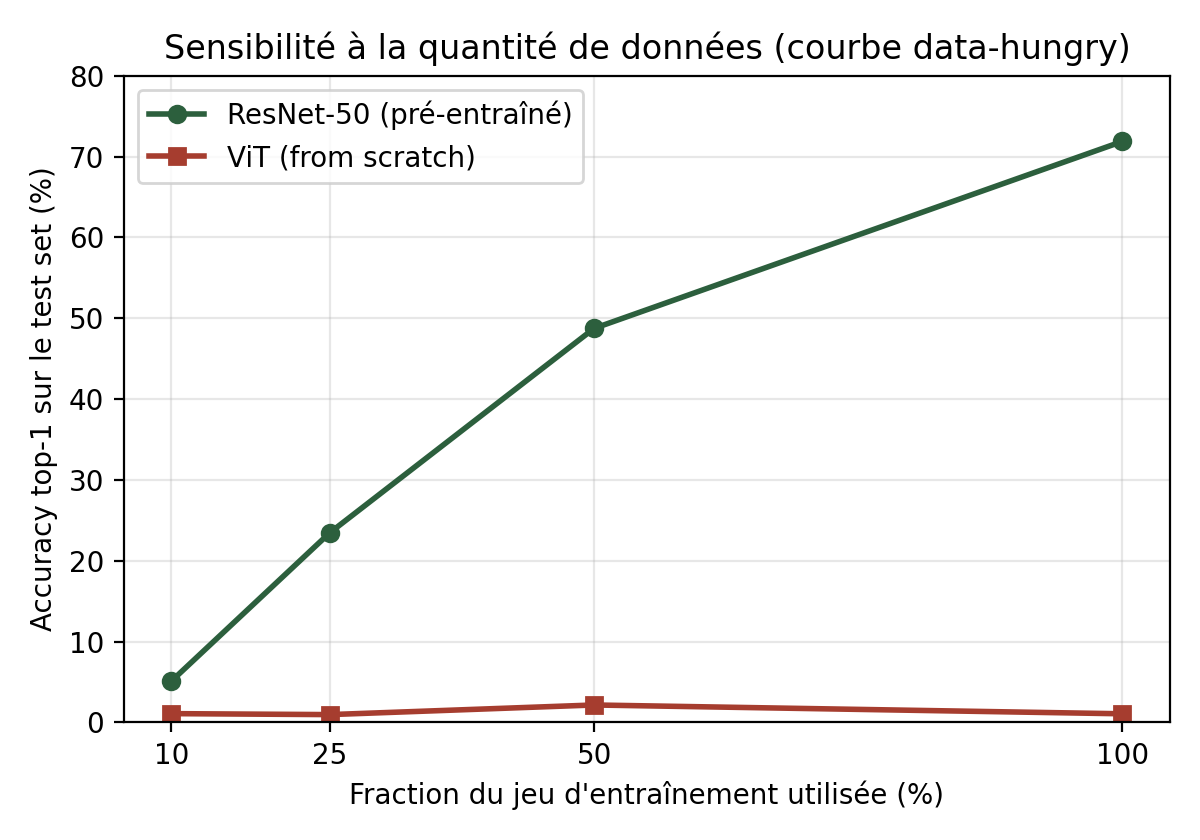
\includegraphics[width=\linewidth]{figures/data_hungry_curve.png}
  \caption{Accuracy top-1 en fonction de la fraction du jeu d'entraînement utilisée, pour ResNet-50 et le ViT from scratch.}
  \label{fig:data_hungry}
\end{figure}

\subsection{Discussion des résultats}

Trois observations principales se dégagent de cette étude d'ablation.

\textbf{Le pré-entraînement est déterminant pour le ViT.} Le ViT
pré-entraîné sur ImageNet (variante patch32) atteint 53{,}9\,\% de
top-1, largement au-dessus du ViT from scratch, quelle que soit la
quantité de données d'entraînement disponible pour ce dernier. Ce
résultat confirme empiriquement, sur CUB-200-2011, le comportement
data-hungry du ViT documenté par Dosovitskiy et al.~\cite{dosovitskiy2020vit}
et discuté par Touvron et al.~\cite{touvron2021deit} : sans
pré-entraînement à grande échelle, l'absence de biais inductif de
localité empêche le ViT d'apprendre une représentation utile avec
seulement 5\,094 images d'entraînement.

\textbf{ResNet-50 reste compétitif même avec peu de données.} Grâce à
son biais inductif convolutif, ResNet-50 continue d'apprendre une
représentation exploitable même à 10\,\% des données (5{,}1\,\%
d'accuracy, contre le niveau du hasard pour le ViT from scratch dans
les mêmes conditions), et progresse de façon régulière jusqu'à 71{,}9\,\%
avec le jeu complet.

\textbf{Écart inattendu entre les deux variantes de ViT pré-entraîné.}
La variante patch16 du ViT pré-entraîné (9{,}9\,\%) performe nettement
moins bien que la variante patch32 (53{,}9\,\%), alors qu'un patch plus
fin devrait en théorie capturer des détails plus locaux, utiles pour
une tâche fine-grained. Cet écart suggère un sous-entraînement de la
variante patch16 plutôt qu'une limite intrinsèque de l'architecture, et
constitue une limite identifiée de cette étude (Section~\ref{sec:discussion}).